\subsubsection{UC5 - Scelta della \glo{visualizzazione}}
\begin{figure}[h]
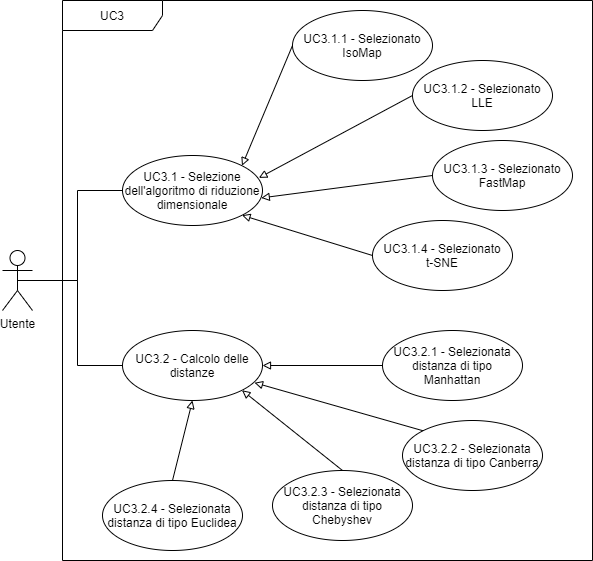
\includegraphics[width=\linewidth]{section/Images/UC3.png}
\centering
\caption{UC5 - Scelta della visualizzazione}
\end{figure}
\begin{itemize}
	\item \textbf{Attore primario}: Utente.
	\item \textbf{Precondizioni}: L'utente ha caricato dei dati nel sistema [UC1] e ha selezionato le dimensioni da utilizzare [UC2].
	\item \textbf{Postcondizioni}: Viene mostrata la visualizzazione scelta, con possibilità di personalizzazione. La scelta viene salvata nel sistema.
	\item \textbf{Scenario principale}:
\begin{enumerate}
	\item	L'utente seleziona una delle seguenti opzioni disponibili:
		\begin{enumerate}[(a)]
			\item \glo{\textit{Scatter Plot Matrix}} [UC5.1]
			\item \glo{\textit{Heat Map}} [UC5.2]
			\item \glo{\textit{Force Field}} [UC5.3]
			\item \glo{\textit{Proiezione Lineare Multi Asse}} [UC5.4]
		\end{enumerate}
\end{enumerate}
	\item \textbf{Estensioni}:
	\begin{enumerate}[(a)]
		\item Nel caso in cui non è stato caricato alcun dato o non è stata scelta alcuna dimensione:
		\begin{enumerate}[1.]
			\item Il grafico non viene visualizzato;
			\item Viene visualizzato un errore esplicativo [UC18].
		\end{enumerate}
	\end{enumerate}
\end{itemize}